\chapter{Anwendungen von Predictive Analytics im öffentlichen Sektor}

% Auswahl
% TODO Fallstudien einfach ausführlichere Beispiele

\section{Daten}

% TODO
% 2 grundlegende Probleme
% - Datenschutz: Achtung Privatsphäre + Angst vor Missbrauch
% - Verzerrungen in Daten: insb. auch Big Data, Daten nicht repräsentativ,
%     Daten kulturabhängig

\section{Öffentliche Verwaltung}

% TODO
% Daten in der öffentlichen Verwaltung
% Open Data Portale ( GovData.de )
% Abgrenzung zu 'Nowcasting'
% Predictive Analytics in Finanzbehörden
% Predictive Policing
% Einschätzung der politischen Stimmungslage
% Vorhersage kultureller Unterschiede

% wackeligste Stimmen identifizieren und sie bei der Wahlwerbung zu priorisieren

% TODO Daten (-> Heise) 
% Thapa_Parycek S. 46

\subsection{Predictive Analytics in der Steuerverwaltung}

Hier \cite{OECD}.


Die Anwendungen von Predictive Analytics in der Steuerverwaltung werden in einer
Studie des \emph{Forum on Tax Administration} (FTA) diskutiert\footnote{
Deutschland ist bei dieser Studie allerdings nicht dabei.
}. Der folgende Text beschreibt diese Anwendungsfälle.

\subsubsection{Audit Case Selection}

Steuerbehörden führen Kontrollen von Unternehmen und Personen durch, um Steuerbetrug
aufzudecken und zu verringern. Um verfügbare Ressourcen besser einzusetzen, werden mit Hilfe
von Predictive Analytics die Fälle für die Prüfung priorisiert, bei denen der größte Betrugsverdacht
besteht.
% TODO

% FTA: Forum on Tax Administration Survey (DE leider nicht dabei)

% EINSATZGEBIETE VON PA

% 1) Audit Case Selection

% hauptsächliches Anwendungsgebiet (S. 20)
%  prioritise cases for investigation, audits

%  social network analysis (für bestimmte fälle, z. B. VAT carousel fraud)(S. 21-22)
% identify risk groups where individual-level assessments may fail
% identify links between individuals, assemble connected individuals to visualised networks
% Analyse der networks (risk score) per Hand, rule based oder statistical model

% 2) Filing (Aktenablage) and payment compliance (S. 24)

% aim: secure outstanding payment or return or prevent the problem from occurring
% predictive: identify taxpayers who are likeliy to fail to meet their obligations
% prescriptive: how communicate most effectively with this group

% 3) Debt management (S. 26)

% resource priorization
% traditional: identify groups of potentially high-risk debtors
% new (u. A. uplift modelling): identify cases that are most likely to respond to
%   debt-management intervention

% 4) Taxpayer Service (S. 27)

% z. B. Text mining and sentiment analysis

% Text minining of inbound email in Singapore (S. 27-28)

% identify the nature of taxpayer inquiries
% example: identify common queries of taxpayers after policy has changed
%   -> able to react: infos on website, updates to taxpayers (vorsorglich)
% Text Mining replaced manual tracking of email enquiries + track enquiries more objectively

% 5) Policy evaluation (S. 28)

% most analytics work carried out to support operational decision-making
% but too for decision-making in relation to strategy and policy

% tax gap analysis (Steuerlücke), forecasting the impact of changes in tax policy

% (S. 29) 2012 model (macro-economic) for assessment the effects of tax-reform on economy and social-welfare
% estimate economic and social consequences of tax reform, 
% report of analytics team played a key role in the policy reform process

% DATENPROBLEME

 % S. 51
% concerns about representativeness of data

% data from highly biased samples (alte interventionsfälle) -> nur kleiner ausschnitt aus gesamtpopulation

% selection effects -> biases

 % S. 52

% data from randomly selected audits in US to improve representativeness

% DATA COMPREHENSIVENESS (S. 52)

% data for analytics project from data collected and stored for
%   operational purposes

% -> missed opportunities: not useful information for operational purposes
%     (e. g. type of non-compliance in audit) but would be useful for analytical purposes
%     distinct models for each risk type possible

\subsection{Predictive Policing}

Grafik aus \cite{Bode}, S.~2.

\begin{figure}%[!hbt]
\centering
\caption{Predictive Policing Prozess}
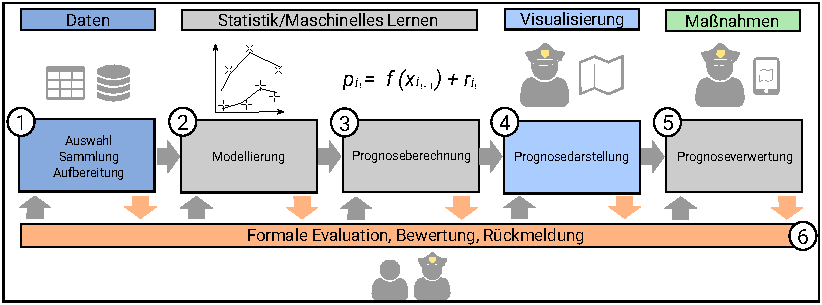
\includegraphics[scale=1.1]{Grafiken/Predictive_Policing_Ink.pdf} 
\label{pic:Predictive_Policing}
\end{figure}

\subsection{Weitere Anwendungen}

\subsection{Cambridge Analytica - Fallstudie}

\begin{figure}%[!hbt]
\centering
\caption{Nutzung von Facebook Likes zur Vorhersage von Nutzerattributen}
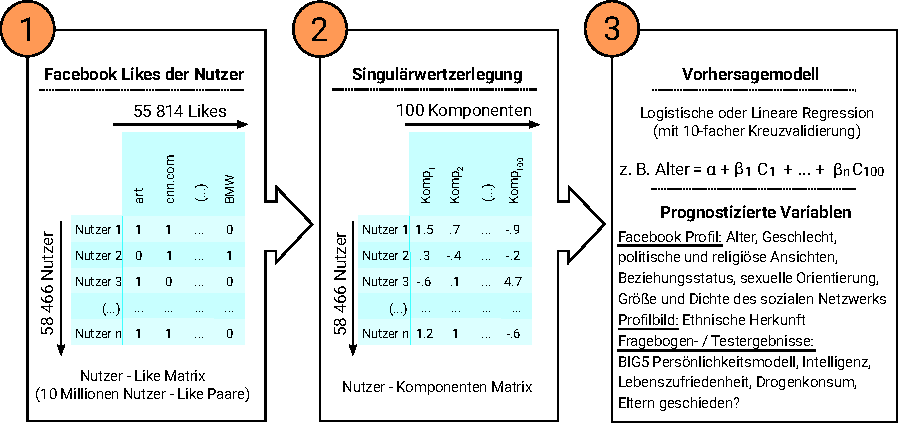
\includegraphics[scale=1.0]{Grafiken/Facebook_Likes_Ink.pdf} 
\label{pic:Like_Matrix}
\end{figure}

\section{Gesundheit}

Diese Haltung war überraschend genug, um eine Nachfrage des Journalisten
auszulösen.

% TODO
% Google Flu Trends (vorerst gescheitert)
% Kohortenstudien nützlich bei: bsp. Kampagnen zur öffentlichen Gesundheit
%   bsp. Ernährungskampagnen, Anti-Rauch-Kampagnen 
% Kohortenstudien: nicht persönlich (s. Watson, Abschnitt Cohort treatment),
%   aber Sicherheitsbedenken bleiben (Anonymisierung nicht möglich, Sicherheits
%   risiken ...)
\subsection{Flint Trinkwasserskandal - Fallstudie}

\section{Bildung}

% Anwendungsbeispiel Decision Tree
